\documentclass[12pt, handout=show,notes=show]{beamer}
\usetheme[width=0cm]{Goettingen}
\usecolortheme{rose}
\useoutertheme{default}

\usepackage{hyperref}
\usepackage{fontspec} 
\setsansfont{Futura LT}
%\setmonofont[Scale=0.8]{Monaco} 


\usepackage{arydshln}

%\usefonttheme{serif}
%%%%lualatex on

%\usepackage{fontspec}
%%\setmainfont{EBGaramond12-Regular.otf}[
%%    SlantedFont = EBGaramond12-Regular.otf ,
%%    SlantedFeatures = {FakeSlant} ,
%%    ItalicFont  = EBGaramond12-Italic.otf ,
%%]
\usepackage{amsmath}
%Ligatures={Contextual, Common, Historical, Rare, Discretionary}
%\setmainfont[Mapping=tex-text]{Linux Libertine O}

\usepackage{mathptmx}
\usepackage{latexsym}
\usepackage{mathtools}
\usepackage{multirow}


\DeclarePairedDelimiter\abs{\lvert}{\rvert}%
\DeclarePairedDelimiter\norm{\lVert}{\rVert}%


\makeatletter
\let\oldabs\abs
\def\abs{\@ifstar{\oldabs}{\oldabs*}}
\let\oldnorm\norm
\def\norm{\@ifstar{\oldnorm}{\oldnorm*}}
\makeatother

\title{
	Winter Simulation Conference:\\
	Co-evolution of trade and culture.
}

\date{6-11th of December 2016}

\author{Simon Carrignon, Jean-Marc Montanier \& Xavier Rubio-Campillo}
\begin{document}
\begin{frame}
	\maketitle

\end{frame}

\section{Introduction}
\begin{frame}{Introduction}
    EPNet, an European Reasearch Council's Grant that:\\
    \begin{quote}
    \small
    ``project and intends to set up an innovative framework to investigate the \textbf{political and economical} mechanisms that characterised the dynamics of the commercial trade system during the Roman Empire''\\
	\emph{EPNet Website (www.epnet.org)}
    \end{quote}
    \begin{center}
    \end{center}
	\begin{center}
		
\includegraphics[height=2.5cm]{images/epnetLogo.png}
	\end{center}
\end{frame}



\section{Context}

\begin{frame}{Once upon a time}

	The Monte Testaccio, an amphora garbage in Roma.\\

	\begin{center}
		\includegraphics[height=0.3\textwidth]{images/Mount-Testaccio.jpg}
		\hfil \includegraphics[height=0.3\textwidth]{images/Mount-Testaccio2.jpg}\\
		\vfill
		\includegraphics[height=0.3\textwidth]{images/titulus.png}

	\end{center}

\end{frame}
\begin{frame}{And all other database}
    
    \begin{center}
	\includegraphics[height=0.8\textwidth]{images/fortGreekPlaceAndAmphora.png}
    \end{center}
\end{frame}

\begin{frame}{Historical question}
	\begin{center}
		\Huge
		What was the nature of the Roman Economy?\\
	\end{center}
	\vfill
	\begin{block}
		{The primitivism/modern debate}
		\begin{center}
		    \em
		    ``Somehow comparable to nowadays economy'' \\
		    \emph{vs}\\
		    ``Not comparable''
		\end{center}
	\end{block}
\end{frame}

\begin{frame}{How to acchieve this?}
	Transdisciplinary approach and quantitative arguments:
	\begin{itemize}
		\item<1->Historical \& Archaeological investigation
		\item<2-> Data integration \& Sparql Ontology
		\item<3-> Complex Sytem \& Network analysis
		\item<4-> Simulation \& Model Testing
	\end{itemize}
	
\end{frame}
\section{ABM Framework}

\begin{frame}{A General Agent Based Framework }
    A tool to test archaeological and historical hypothesis:
	\begin{center}
	    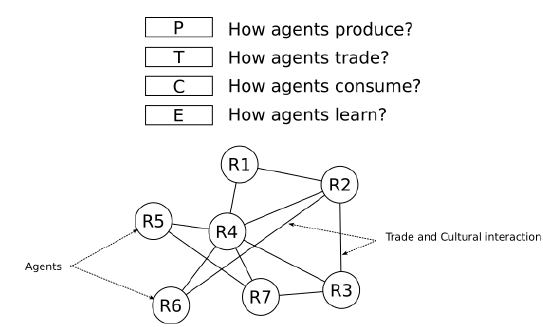
\includegraphics[width=.6\textwidth]{images/schema_model.png}
	\end{center}
\end{frame}


\begin{frame}{}

	\begin{alertblock}{Underlying assumption}
	    \begin{center}
		Cultural mechanisms transorm Economy \\
		\begin{center}
		    $  \scalebox{4}{\circlearrowright}$
		\end{center}
		Changes in Economy influence Culture
	    \end{center}
	\end{alertblock}


\end{frame}


\begin{frame}{Proof of concept}
     Simple known dynamics to illustrate  :
    \begin{enumerate}
	\item a	simple bartering mechanism (Gintis 2009),
	\item a cultural dynamics: ``copy the most successufl'' (Bentley 2006).
    \end{enumerate}
\end{frame}
	
\begin{frame}{The Model}
	\begin{block}{1. Barter Mechanism}
	    \begin{itemize}
		\item Agent 
		    $\left\{
			\begin{tabular}{@{}l@{}}
			    Goods \\
			    Value attributed to each goods\\
			\end{tabular}
			\right.$
		    \item Agents \emph{produce} one good and \emph{exchange} it to obtain the other goods.
		    \item After the exchange, the agents \emph{consume} all goods 
		\end{itemize}

	\end{block}
\end{frame}

\begin{frame}{The Model}
    More details about the model : 
    \vfill
	\begin{block}{2. Evolutionary Dynamics}
	    Every step:
	    \begin{itemize}
		    \item Agent are \emph{ranked} given the result of the consumption.
	    \end{itemize}
		After 10 steps:
		\begin{itemize}
		    \item  Less successful agents \emph{copy} the most successful (Biased-Copy).
		    \item Given a probability $\mu$ the value attributed to some goods is modified (Innovation/Mutation)
		\end{itemize}
	\end{block}
\end{frame}



\section{Results}
\begin{frame}{Results: Random copy vs Success Baised copy :}
    \subsection*{Distribution of variant:}
    \begin{figure}[!h]
	\begin{center}
	    \begin{tabular}{ccc}
		\includegraphics[width=5cm]{../img/2SetupDistribA.pdf}\\
	    \end{tabular}

	\end{center}
	%\caption{Frequencies distribution, where each points represent the mean for 100 runs, for: a) the neutral and the trading models.  b) the neutral model and the trading model without the trading innovation process. c) the trade model and the trade model without the trading innovation process.}
    \end{figure}
\end{frame}

\begin{frame}{Results: Random copy vs Success Baised copy :}
    Evolution of Score
    \begin{figure}[!h]
	\centering
	\begin{tabular}{ c c}
	    Neutral Model & Trading Model \\
	    \includegraphics[width=4cm]{../img/ScoreEvolutionForRandom-G3N500.pdf}
	    & \includegraphics[width=5cm]{../img/ScoreEvolutionForTrade-G3N500.pdf}

	\end{tabular}
	\caption{Evolution of the score within the two different models for two typical run with 500 agents and 3 goods evolving during 10000 timestep.}%%
	\label{fig:scoreEvol}
    \end{figure}
\end{frame}
    


\begin{frame}{Results: Economic Dynamics}
	\begin{figure}
	    \caption{Exemple for 3 goods and 500 agents}
	    \begin{columns}
		\column{.5\textwidth}
		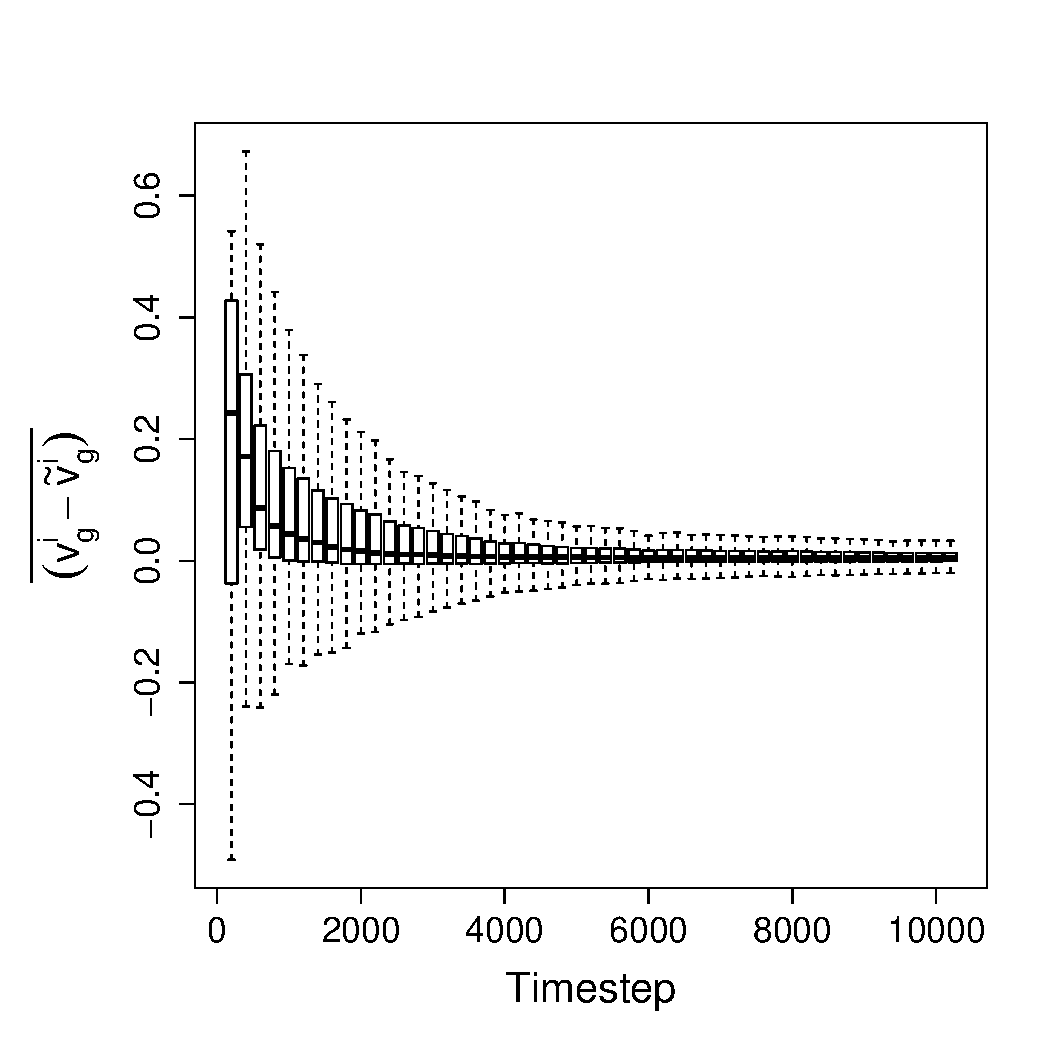
\includegraphics[height=\textwidth]{images/ClearingPriceDistanceEvolutionForTrade-G3N500.pdf}\\
	    \end{columns}
		@~Equilibrium: price $\rightarrow$ optimal prices.
	\end{figure}
	
\end{frame}

\begin{frame}{Next Steps}
    Implementing historical hypothesis and compare results to data and other theoretical exploration:

	\begin{itemize}
		\item Network Topologies (Ongoing)
			\vfil
		\item	Multilevel dynamics (Province vs Economical Agents\ldots)
			\vfil
		\item	Evolution of specialisation 
			\vfil
		\item	\ldots
	\end{itemize}
\end{frame}



\begin{frame}
    \Huge
    Thank for you attention!
\end{frame}


%\section{Computer and Living Systems}
%
%\begin{frame}{Computer and Living Systems}
%    \begin{figure}
%	    \includegraphics[width=.45\textwidth]{images/creatures.jpg}\hspace{.5cm}
%	\includegraphics[width=.45\textwidth]{images/war2.png}
%    \end{figure}
%    Find the good ``rules'' and ``something unexpected'' will happen.
%\end{frame}
%
%\subsection{Biology and Informatics}
%\begin{frame} {Biology and computers}
%
%    \begin{figure}
%	\includegraphics[height=3.5cm]{images/mitosis.png}\hspace{.8cm}
%	\includegraphics[width=2cm]{images/Rule22rand.png} 
%    \end{figure}
%
%    \vfill
%
%    \begin{center}
%	\emph{Why sometime, Computer and Living 'stuff' show similar properties? }
%    \end{center}
%
%\end{frame}
%
%\begin{frame}{Biology and computer}
%
%    Simple rules, simple modifications, complex mechanism\\
%    \begin{figure}
%	\includegraphics[width=3cm]{images/hybrid.png}\hspace{.3cm}
%	\includegraphics[width=3cm]{images/maize.png} \\
%	\includegraphics[width=3cm]{images/tsp.png}
%    \end{figure}
%    
%\end{frame}
%
%\begin{frame}{Biology and computer}
%    \begin{alertblock}	{ A remaining frustration\ldots} 
%	\vfill
%	Feeling like :
%	\vfill
%	\begin{table}
%	    \centering
%	    \begin{tabular}{c|cl}
%		\textbf{Tool} & \textbf{Interest} & \\\cline{1-2}
%		Informatic & Biology &  $\rightarrow$ Biologist using Informatics  \\
%		Biology & Informatic& $\rightarrow$ Computer Scientist using Biology\\
%	    \end{tabular}
%	\end{table}
%    \end{alertblock}
%\end{frame}
%
%\subsection{Cognitive sciences}
%
%\begin{frame}{Neurosciences \& Artificial Intelligence}
%
%    ``Simple'' rules, ``simple'' modifications, more ``complex'' mechanism:\\
%    \begin{figure}
%	\includegraphics[width=6cm]{images/cogscience.jpg}\\
%	\includegraphics[width=4cm]{images/ai.jpg}
%    \end{figure}
%    
%\end{frame}
%
%\begin{frame}{Cognitive Sciences \& Complex Systems}
%    \begin{figure}
%	\includegraphics[width=3.5cm]{images/kauffman.jpg}
%    \end{figure}
%
%    \begin{alertblock}	{'Unification'} 
%	\begin{table}
%	    \centering
%	    \begin{tabular}{c|cl}
%		\textbf{Tool} & \textbf{Interest}  \\\cline{1-2}
%		Informatic & Biology &  $\rightarrow$ Biologist using Informatics  \\
%		Biology & Informatic& $\rightarrow$ Computer Scientist using Biology\\
%	    \end{tabular}
%	\end{table}
%    \end{alertblock}
%\end{frame}
%
%\begin{frame}{Cognitive Sciences \& Complex Systems}
%    \begin{figure}
%	\includegraphics[width=3.5cm]{images/kauffman.jpg}
%    \end{figure}
%    \begin{alertblock}{'Unification' } 
%	\begin{table}
%	    \centering
%	    \begin{tabular}{c:cl}
%		\textbf{Tool} & \textbf{Interest}  \\\cline{1-2}
%		Informatic & Biology &\multirow{2}{*}{{ \LARGE \}} \hspace{.308cm} $\rightarrow$ Complex Systems Scientist}  \\
%		Biology & Informatic& \\
%	    \end{tabular}
%	\end{table}
%    \end{alertblock}
%
%\end{frame}
%
%
%\subsection{Evolutionary Theory}
%
%\begin{frame}{Evolutionary studies}
%	\begin{center}
%		
%	\end{center}
%    \begin{columns}
%	    \begin{column}{.2\textwidth}
%		    \includegraphics[width=.9\textwidth]{images/tsp.png}
%	    \end{column}
%	    \begin{column}{.6\textwidth}
%		    \begin{center}
%			    \includegraphics[width=.4\textwidth]{images/cogscience.jpg}
%		    \end{center}
%		    \begin{exampleblock}{A common way to approach all that?}
%			    Simple rule, simple mechanism, complex dynamics\ldots\\
%			    \begin{itemize}
%				    \item The Theory of Evolution?
%			    \end{itemize}
%		    \end{exampleblock}
%	    \end{column}
%	    \begin{column}{.2\textwidth}
%		    \includegraphics[width=.9\textwidth]{images/hybrid.png}
%	    \end{column}
%    \end{columns}
%
%    \begin{columns}
%	    \begin{column}{.2\textwidth}
%		    \includegraphics[width=.9\textwidth]{images/symbrion-gc1b.png}
%		    
%	    \end{column}
%	    \begin{column}{.2\textwidth}
%		    \includegraphics[width=.9\textwidth]{images/medea-RealRobots.png}
%		    
%	    \end{column}
%	    \begin{column}{.2\textwidth}
%		    \includegraphics[width=.4\textwidth]{images/mitosis.png}
%		    
%	    \end{column}
%    \end{columns}
%    
%    
%\end{frame}
%
%\begin{frame}{Evolutionary Robotics}
%
%	\begin{center}
%		\huge Study of speciation \& specialisation by artificially evolve swarm of robots.\\
%
%		\dots
%	\end{center}
%
%	
%\end{frame}
%
%\begin{frame}{Philosophy of Biology}
%	What am I \emph{really} learning with that? Who will I convince?
%    \begin{itemize}
%	\item What is the Evolutionary Theory?
%	\item How can I study it?
%	\item What are the tools I used and how/why they can help me?
%    \end{itemize}
%    \vfill
%    
%    \begin{block}{How to use artificial model to study Evolutionary Biology}
%	 What is a model? What is a theory? an explanation ? What is the Theory of Evolution? Lamarck? Darwin? Spencer? The Biometricians? Mendelism? The Modern Synthesis? Dawkin? Gould? \ldots 
%    \end{block}
%
%    \begin{figure}
%	\includegraphics[width=3.5cm]{images/darwinianspace.png}
%	\caption{From Godfrey-Smith 2009}
%    \end{figure}
%
%    
%\end{frame}
%
%
%\begin{frame}{And with all that?}
%
%    \begin{center}
%	\huge
%	A huge mess, a lot of knowledge, but\ldots\\  \textbf{no MBA}!
%    \end{center}
%
%
%    
%\end{frame}
%\begin{frame}
%    An ERC grant, 2 dynamics research center, 4 years of PhD, an amazing case study :
%    \vfill
%
%    \begin{center}
%	\huge
%	The evolution of Economy and Culture in the Roman Empire.\\
%	\vfill
%	\small
%	(ERC advanced grant : Production and Distribution of Food during the Roman Empire: Economic and Political Dynamics EPNET)
%    \end{center}
%\end{frame}
%
\end{document}


